\documentclass[10pt,a4paper]{article}

\usepackage{polski}
\usepackage[utf8]{inputenc}

\usepackage[polish]{babel}
\usepackage{hhline}
\usepackage{pgfplots}

\usepackage{multicol}
%\usepackage{slashbox}
\usepackage{graphicx}
\usepackage{caption}
\usepackage{subcaption}
\usepackage{colortbl}

\usepackage{geometry}
\geometry{a4paper, total={170mm,257mm}, left=20mm, top=20mm }

\author{Jan Techner 132332 i Sebastian Maciejewski 132275 \\ grupa I1}
\title{Analiza zdjęć - \\ rozpoznawanie par symboli na kartach Dobble}
\date{18 listopada 2018}
\setlength{\parindent}{0pt}
\newcommand{\forceindent}{\leavevmode{\parindent=3em\indent}}
\begin{document}
\maketitle

\section{Wstęp}

\forceindent Program, który napisaliśmy ma za zadanie pobrać od użytkownika zdjęcie stanu rozgrywki (od 2 do 5 graczy) i zaznaczenie na tym zdjęciu identycznych symboli występujących na różnych kartach. \\
Nasz algorytm rozpoczyna pracę od podziału zdjęcia na pojedyncze karty, dodania dla każdej karty listy rozpoznanych na niej symboli, a następnie umieszczenia karty w 
liście wyciętych kart. Ten fragment programu jest kluczowy dla końcowego rezultatu, bowiem to od jakości rozpoznania kart i symboli zależy skuteczność ich porównywania. \\

W skrócie: proces wycinania polega na znalezieniu krawędzi po zastosowaniu filtru threshold dla zdjęć z ciemnym tłem lub specjalnego filtru threshold po 3 kanałach R, G, B (który to filtr pozwala uzyskać wyjątkowo dokładne obrysy, ponieważ analizuje każdy kanał z osobna, następnie złączając je w jeden obraz) dla zdjęć z jasnym (białym) tłem. W przypadku ciemnego tła symbole są przyporządkowywane do kart dzięki algorytmowi wykrywania konturów, który zwraca drzewiastą sktrukturę. Na jej podstawie można rozpoznać czy symbol zawiera się w karcie. Ponowne zastosowanie filtru threshold, tym razem w wersji RGB na jednej wyciętej karcie, umożiwia dokładne rozpoznawanie symboli po powtórnym wywołaniu algorytmu wyszukiwania konturów. W przypadku zdjęć z jasnym tłem algorytm wykrywania konturów zwraca same symbole, które następnie są grupowane w karty na podstawie ich wzajemnych odległości na zdjęciu - w ten sposób mamy możliwość wykrycia kart mimo niekontrastowego tła zdjęcia. Tak rozpoznane symbole są zapisywane jako małe wycinki zdjęcia (najmniejsze prostokąty, w których mieści się symbol) w tablicy symboli dla danej karty. \\

Kiedy już uda się wyciąć karty i symbole, przychodzi czas na porównywanie ich ze sobą - w tym celu dla każdej pary kart (co można, nie zmniejszając ogólności rozumowania, sprowadzić do przypadku porównywania każdej karty poza najbliższą środkowi zdjęcia z tą najbardziej środkową kartą) wywoływana jest funkcja porównująca, której zadaniem jest zaznaczenie na oryginalnym zdjęciu pary symboli, które odpowiadają sobie na tej parze kart. 

Działanie funkcji porównującej można rozłożyć na kilka etapów - na początek przechodzi ona po wszystkich parach symboli i oblicza różnice momentów hu, wartości kolorów (w HSV) i stosunku długości boków (najmniejszego prostokąta zawierającego cały symbol) dla każdej pary. Jeśli różnica momentów i stosunku długości jest w ustalonym przedziale akceptowalnych dopasowań, to taka para symboli jest zapisywana jako potencjalnie prawidłowe dopasowanie. Następnie dla wszystkich takich dopasowań porównywane są różnice kolorów symboli i te, których różnica kolorów jest najmniejsza są uznawane za prawidłowe dopasowanie. Między środkami tych symboli jest rysowana strzałka na głownym zdjęciu, co ma oznaczać, że te dwa symbole są identyczne z dokładnością do rozmiaru i rotacji.

\newpage

\section{Przetwarzanie - analiza przypadków}
Przyjrzyjmy się dokładniej procesowi przetwarzania w kilku przypadkach.
\subsection{Pięciu graczy, ciemne tło, naturalne oświetlenie}
Na podstawie poniższego zdjęcia oczekujemy, że program odnajdzie wszystkie 12 dopasowań z zadowalającą dokładnością:\\
\begin{center}
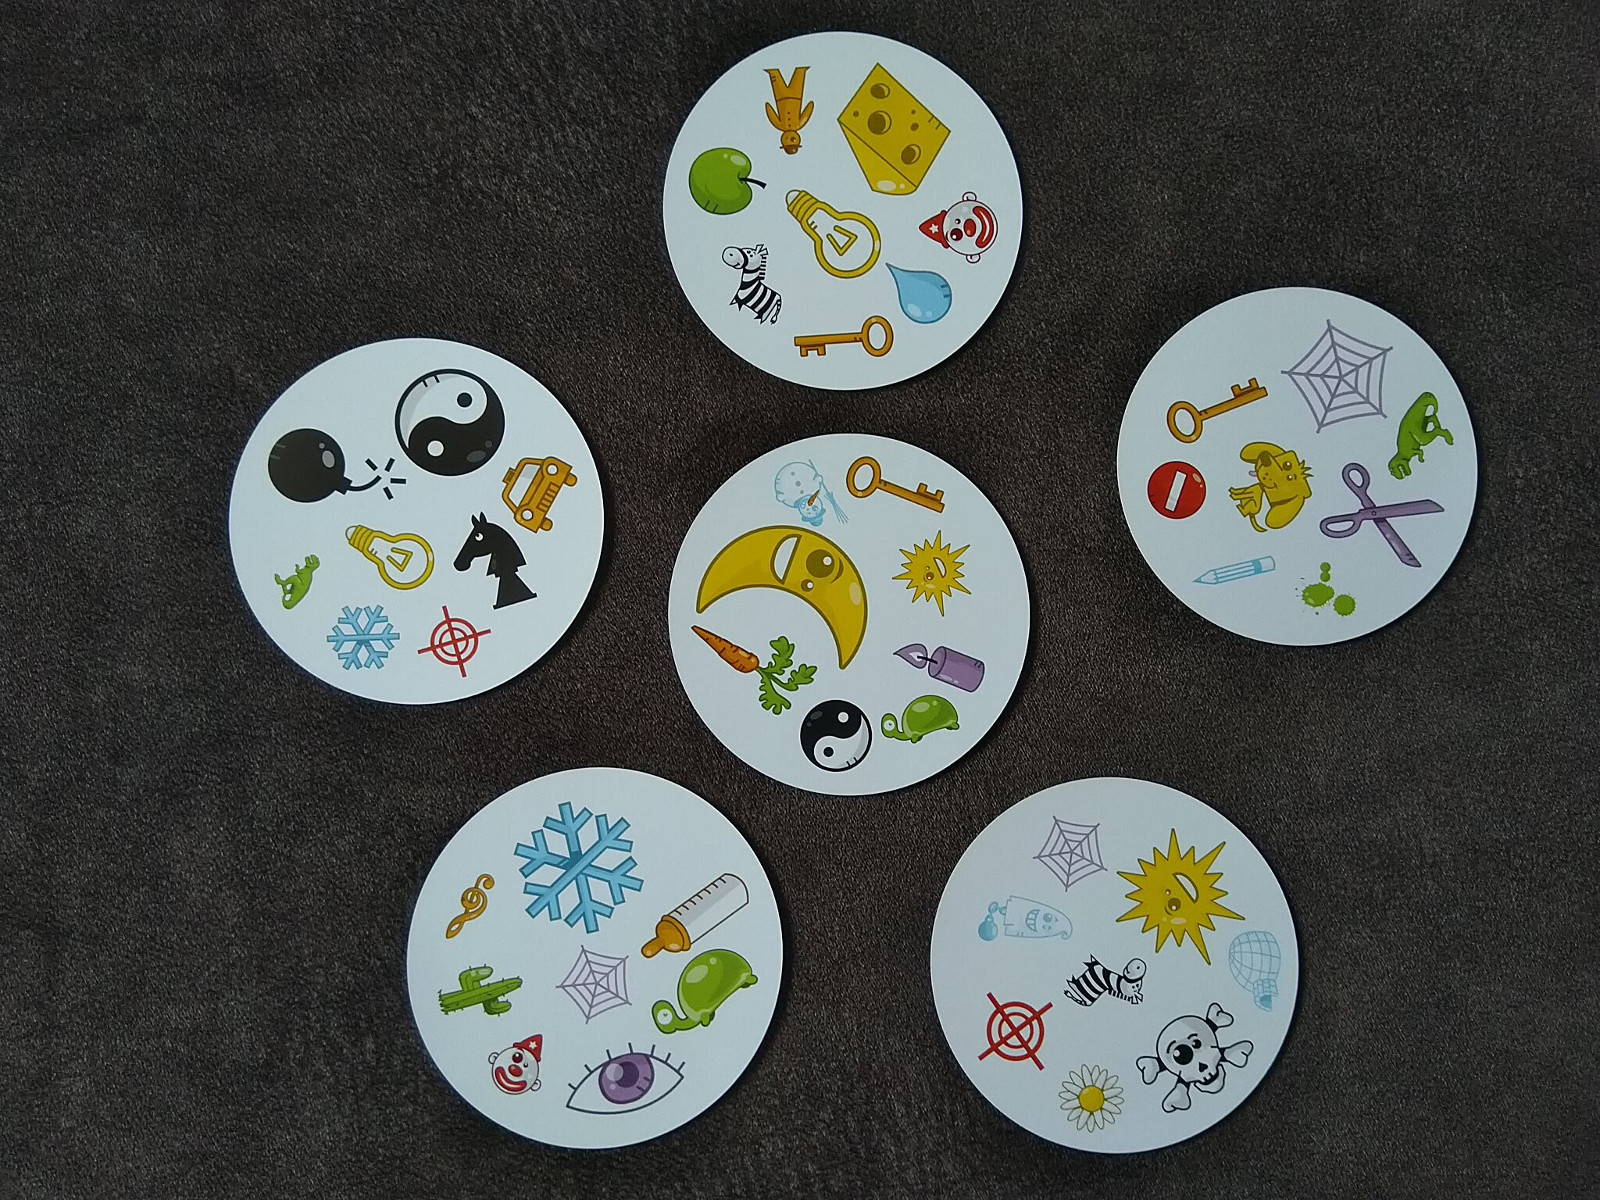
\includegraphics[scale=0.25]{2.1/dobble04.jpg}
\end{center}
Najpierw zajmujemy się wycięciem wszystkich 6 kart i wybieleniem tła (w celu prostszego użycia filtru threshold na późniejszym etapie przetwarzania). Nasza tablica kart zawiera teraz takie karty:\\
\begin{center}
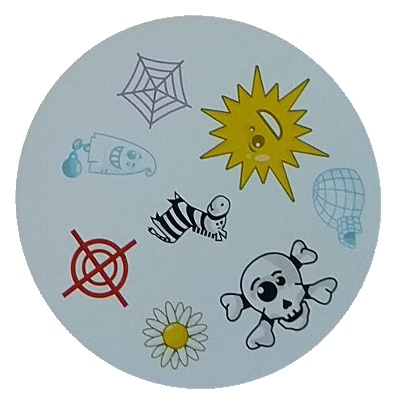
\includegraphics[scale=0.25]{2.1/card0.jpg}
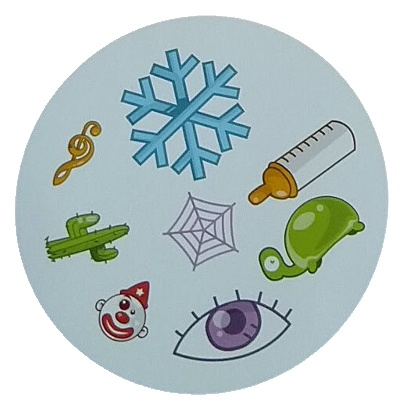
\includegraphics[scale=0.25]{2.1/card1.jpg}
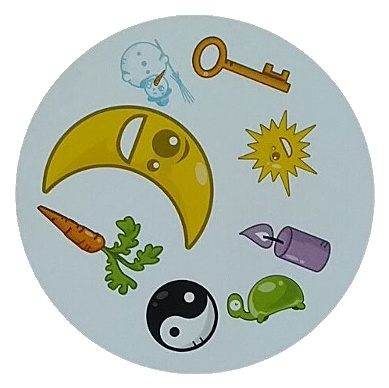
\includegraphics[scale=0.25]{2.1/card2.jpg}
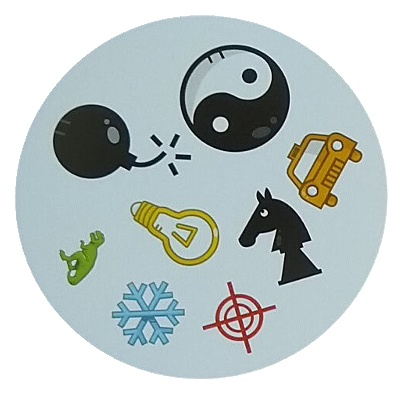
\includegraphics[scale=0.25]{2.1/card3.jpg}
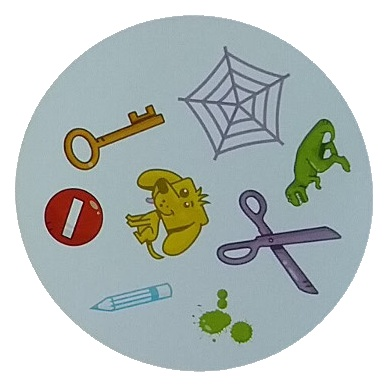
\includegraphics[scale=0.25]{2.1/card4.jpg}
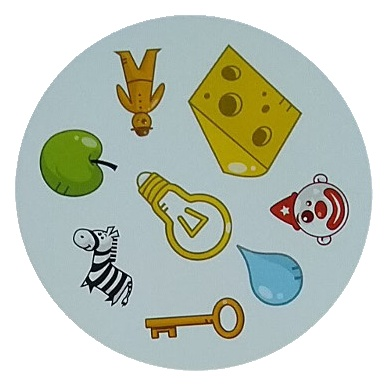
\includegraphics[scale=0.25]{2.1/card5.jpg}
\end{center}
\newpage
Następnie do każdej karty stosujemy threshold RGB, żeby następnie móc odnaleźć kontury symboli. Obrazy, na których szukamy konturów wyglądają w tej chwili tak:\\
\begin{center}
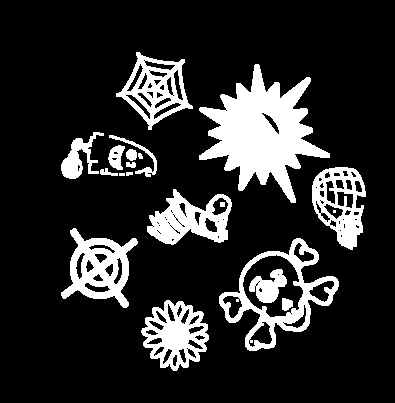
\includegraphics[scale=0.25]{2.1/0.jpg}

\includegraphics[scale=0.25]{2.1/1.jpg}

\includegraphics[scale=0.25]{2.1/2.jpg}

\includegraphics[scale=0.25]{2.1/3.jpg}

\includegraphics[scale=0.25]{2.1/4.jpg}
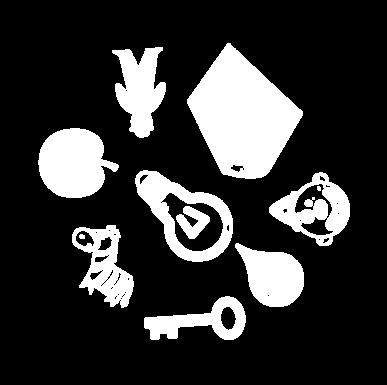
\includegraphics[scale=0.25]{2.1/5.jpg}
\end{center}
Po odnalezieniu konturów każdego symbolu i wycięciu najmniejszego prostokąta w którym się on znajduje, otrzymujemy zbiór kształtów, np. dla pierwszej karty jest to:\\
\begin{center}

\includegraphics[scale=0.5]{2.1/sign00.jpg}

\includegraphics[scale=0.5]{2.1/sign01.jpg}

\includegraphics[scale=0.5]{2.1/sign02.jpg}

\includegraphics[scale=0.5]{2.1/sign03.jpg}

\includegraphics[scale=0.5]{2.1/sign04.jpg}

\includegraphics[scale=0.5]{2.1/sign05.jpg}

\includegraphics[scale=0.5]{2.1/sign06.jpg}

\includegraphics[scale=0.5]{2.1/sign07.jpg}

\includegraphics[scale=0.5]{2.1/sign08.jpg}
\end{center}
Jak widać jest problem z symbolem duszka, który podzielił się na dwa znaki - jasną, prawie białą górę i niebieski dół. Nie powinno to sprawiać problemów na dalszym etapie przetwarzania o ile wszystkie duszki na zdjęciu zachowają się w podobny sposób - wówczas porównamy np. jedynie dolne części. Pozostaje jeszcze usunąć (wybielić) niepotrzebne tło obrazków. Po tym etapie przetwarzania wiemy, że pierwsza karta składa się z następujących symboli:
\begin{center}
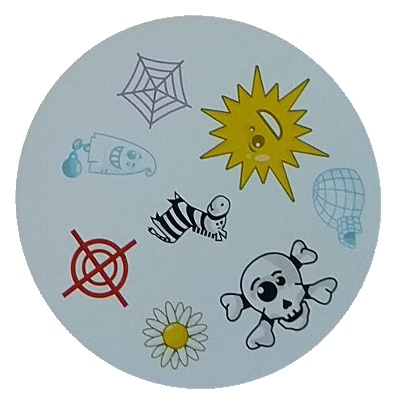
\includegraphics[scale=0.4]{2.1/card0.jpg} \\

\includegraphics[scale=0.5]{2.1/card0sign0.jpg}

\includegraphics[scale=0.5]{2.1/card0sign1.jpg}

\includegraphics[scale=0.5]{2.1/card0sign2.jpg}

\includegraphics[scale=0.5]{2.1/card0sign3.jpg}
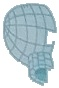
\includegraphics[scale=0.5]{2.1/card0sign4.jpg}

\includegraphics[scale=0.5]{2.1/card0sign5.jpg}

\includegraphics[scale=0.5]{2.1/card0sign6.jpg}

\includegraphics[scale=0.5]{2.1/card0sign7.jpg}

\includegraphics[scale=0.5]{2.1/card0sign8.jpg}
\end{center}

\newpage
Na tym etapie pozostaje już tylko wywołanie funkcji dopasowywania dla wszystkich znalezionych kart - po jej wywołaniu otrzymujemy następujący obraz:
\begin{center}
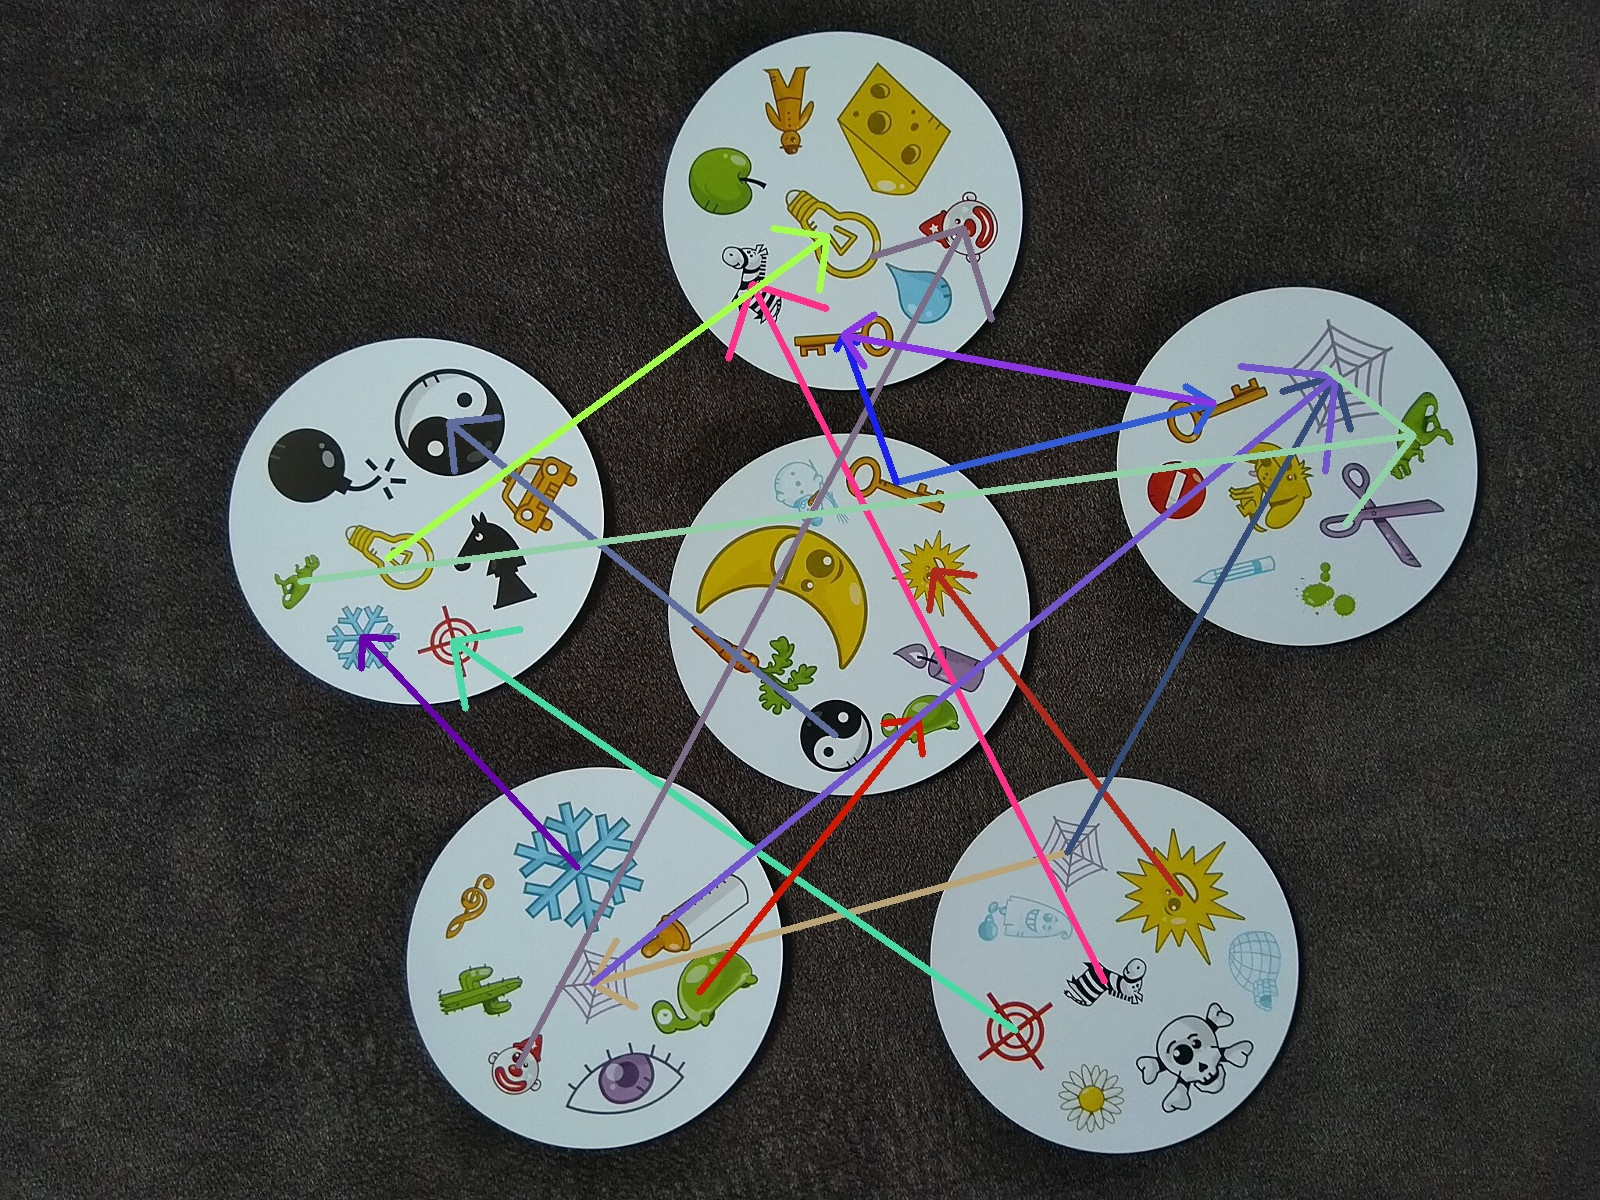
\includegraphics[scale=0.25]{2.1/img_arrows0.jpg}
\end{center}
Jak widać, w tym przypadku udało się odnaleźć 100\% dopasowań.

\section*{Wnioski}
\forceindent Porównanie zapisanych widm z tablicami spektralnymi pokazuje, że w lampach A-C znajdują się następujące pierwiastki chemiczne :
\begin{center}
\begin{tabular}{|c|c|c|c|c|c|}
\multicolumn{2}{c}{Lampa A} & \multicolumn{2}{c}{Lampa B} & \multicolumn{2}{c}{Lampa C}\\
\hline
$\lambda (nm)$ & Natężenie & $\lambda (nm)$ & Natężenie & $\lambda (nm)$ & Natężenie\\
\hline
485,3 & b. małe & 387,8 & duże & 585,8 & b. duże\\
\hline
655,9 & duże & 446,5 & średnie & 594,3 & małe \\
\hline
750,3 & b. duże & 500,7 & duże & 609,3 & średnie \\
\hline
763,2 & średnie & 589,0 & b. duże & 614,3 & duże \\
\hline
810,9 & średnie & 667,3 & b. duże & 625,7 & małe \\
\hline
814,5 & małe & 706,2 & b. duże & 633,2 & małe \\
\hline
&& 728,2 & średnie & 639,9 & b. duże \\
\hline
&&&& 650,2 & średnie \\
\hline
&&&& 655,9 & małe \\
\hline
&&&& 667,3 & małe \\
\hline
&&&& 692,3 & b. małe \\
\hline
&&&& 703,3 & małe \\
\hline

\end{tabular}
\end{center}
\begin{center}
\begin{tabular}{|c|c|}
\hline
\textbf{Lampa} & \textbf{Pierwiastek} \\
\hline
A & Argon \\
\hline
B & Hel \\
\hline
C & Neon \\
\hline
\end{tabular}
\end{center}

\forceindent Jak widać na powyższych wykresach, maksymalne pasma spektralne dla lampy 1. położone są między $ 542,3 - 545,5 nm$ i $612,1 nm$, a dla lampy 2. w $459,0 nm$. Dla lampy 3. położenie pasm jest różne w zależności od koloru, zaś dla lampy 4. pasmo jest identyczne dla każdego natężenia prądu, zmienia się jedynie intensywność świecenia.\\

\forceindent Dodatkowo, po porównaniu widama lampy 1. z tablicą spektralną rtęci, można zauważyć, że intensywności dla odpowiednich długości fali, przedstawione w tabeli, bardzo dobrze pokrywają się z wykresem, co pokazuje, że pierwiastkiem emitującym światło w świetlówkach kompaktowych jest rtęć. \\

\forceindent Przeprowadzone doświadczenie unaocznia różnicę między różnymi rodzajami światła. Różnice te wynikają z tego, że różne żarówki wykonane są z różnych pierwiastków, co widać szczególnie w przypadku lamp A, B i C. Różnica w widmach wynika z różnic w długości fali światła wpadającego do spektrometru, co gołym okiem widać na przykładzie lampy 3., której różne barwy światła różniły się znacząco swoimi widmami. Doświadczenie wykorzystujące lampę 4. ukazuje, że intensywność świecenia, jak można było przewidzieć, nie wpłynie w sposób zauważalny na zakres pasma światła, zmieni się jedynie intensywność światła.

\end{document}